\section{Model}
%%%%%%%%%%%%%%%%%%%%%%%%%%%%%%%%%%%%%%%%%%%%%%%%%%%%%%%%%%%%%%%%%%%%%%%%%%%%%%%%%%%%%%%%%%%%%%%%%%%%%%%%%%
\subsection{Data}
\frame
{
\frametitle{Data}
\begin{block}{}
\begin{itemize}
    \item
Sandia has provided MD simulation results which we will use as training data for our ML models. 
\end{itemize}
\end{block}

\begin{block}{}
\begin{itemize}
    \item Two types of boundary conditions for simulations:
    \begin{itemize}
        \item Fully Periodic
        \item Free Surfaces
    \end{itemize}
\end{itemize}
\end{block}
}
%%%%%%%%%%%%%%%%%%%%%%%%%%%%%%%%%%%%%%%%%%%%%%%%%%%%%%%%%%%%%%%%%%%%%%%%%%%%%%%%%%%%%%%%%%%%%%%%%%%%%%%%%%
\frame
{
\frametitle{Descriptors}
\begin{block}{}
Data includes descriptors such as:
\begin{itemize}
    \item $x, y, z$ coordinates for each atom
    \item charge
    \item stress tensor
    \item bond connectivity
    \item newly formed/broken bonds
    \item Coordination number
    \item Number of bridging oxygens
    \item Volume surrounding atom
\end{itemize}
\end{block}
}
%%%%%%%%%%%%%%%%%%%%%%%%%%%%%%%%%%%%%%%%%%%%%%%%%%%%%%%%%%%%%%%%%%%%%%%%%%%%%%%%%%%%%%%%%%%%%%%%%%%%%%%%%%
\subsection{Representations}
\frame{
\frametitle{Representations}

\begin{minipage}[0.2\textheight]{\textwidth}
\begin{columns}[T]
    \begin{column}{0.5\textwidth}
    \vspace{2em}
    To achieve our goals, we will use the following representations to build the machine learning model:
    \begin{itemize}
    \item Graph Representations
    \item Feature Description
    \begin{itemize}
        \item Local Topological Feature
        \item Global Topological Feature
        \item Physical Feature
    \end{itemize}
    \item Extracting Ground Truth
    \end{itemize}
    \end{column}
    
    \begin{column}{0.5\textwidth}
    \vspace{2em}
    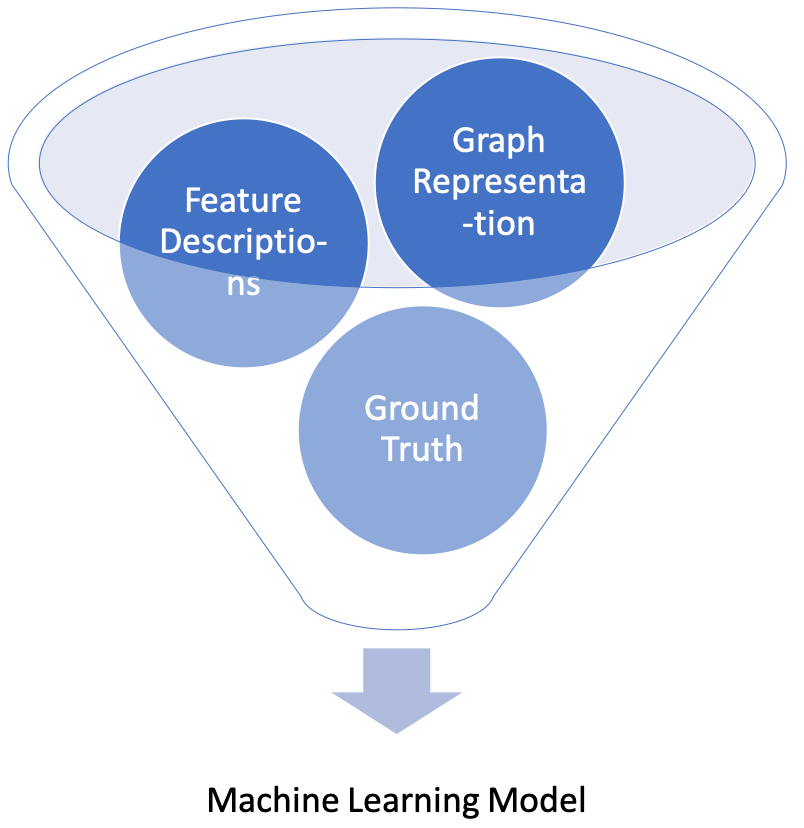
\includegraphics[width=5.5cm]{images/rep.png}
    \end{column}
\end{columns}
\end{minipage}
}


%%%%%%%%%%%%%%%%%%%%%%%%%%%%%%%%%%%%%%%%%%%%%%%%%%%%%%%%%%%%%%%%%%%%%%%%%%%%%%%%%%%%%%%%%%%%%%%%%%%%%%%%%%


\begin{frame}[t]{Graph Representations}
We propose three possible graph representations $G(t)=(V(t),E(t))$, where
$V(t)$ and $E(t)$ represent the set of vertices and edges at time $t$, respectively.

 \begin{columns}[t]
 
   \column{0.3\textwidth}
   \begin{block}{Basic Graph}
   \begin{itemize}
   \begin{footnotesize}
       \item $V$: Si, O atoms
       \item $E$: Chemical bond between atoms
    \end{footnotesize}
    \end{itemize}
    \begin{figure}
	    \centering
        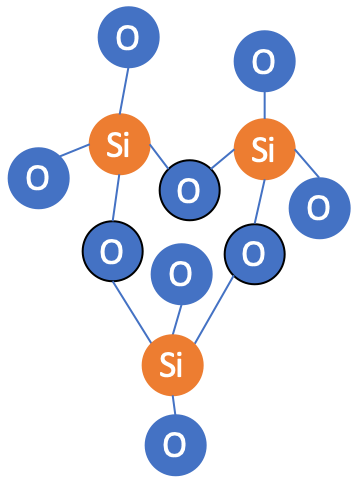
\includegraphics[width=.5\textwidth]{images/basic.png}
	\end{figure}
   \end{block}
   
   \column{0.3\textwidth}
   \begin{block}{Reduced Graph}
   \begin{itemize}
   \begin{footnotesize}
       \item $V$: Si atoms
       \item $E$: Bridging oxygens
    \end{footnotesize}
   \end{itemize}
    \begin{figure}
	    \centering
        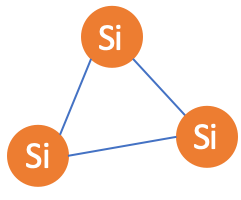
\includegraphics[width=.5\textwidth]{images/reduced.png}
	\end{figure}
   \end{block}
   
   \column{0.3\textwidth}
   \begin{block}{Topological Graph}
   \begin{itemize}
   \begin{footnotesize}
       \item $V$: Rings (closed paths)
       \item $E$: Bridging oxygen
    \end{footnotesize}
   \end{itemize}
    \begin{figure}
	    \centering
        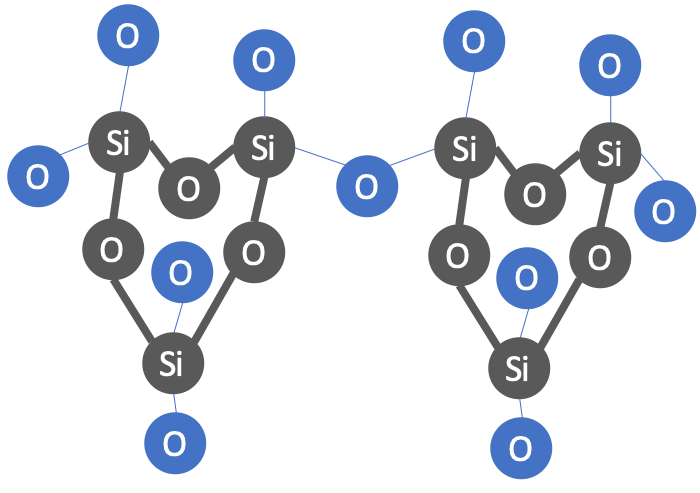
\includegraphics[width=.5\textwidth]{images/ring.png}
	\end{figure}   
   
   
   \end{block}
   
 \end{columns}
\end{frame}

%%%%%%%%%%%%%%%%%%%%%%%%%%%%%%%%%%%%%%%%%%%%%%%%%%%%%%%%%%%%%%%%%%%%%%%%%%%%%%%%%%%%%%%%%%%%%%%%%%%%%%%%%%
\frame
{\frametitle{Feature Description}
\begin{block}{}
\begin{itemize}
    \item Local Topological Features
    \item Global Topological Features
    \item Physical Features
\end{itemize}

\end{block}
}

%%%%%%%%%%%%%%%%%%%%%%%%%%%%%%%%%%%%%%%%%%%%%%%%%%%%%%%%%%%%%%%%%%%%%%%%%%%%%%%%%%%%%%%%%%%%%%%%%%%%%%%%%%
\frame{
\frametitle{Example of Local Topological Features}
\begin{block}{}
\textbf{Number of Bridging Oxygens:} In a Q$_n$ unit, an Si atom is surrounded by $n$ bridging O atoms, each forming an Si–O–Si group. The value of $n$ supplies crucial network connectivity information.
\begin{itemize}
    \item The number of bridging oxygens is equivalent to the degree of a vertex
    \item ML algorithms benefit from having bridging oxygens as an explicit feature
\end{itemize}
\end{block}

%\begin{block}{}
%k-th neighbor quantities. %See SOW
%\end{block}
}
%%%%%%%%%%%%%%%%%%%%%%%%%%%%%%%%%%%%%%%%%%%%%%%%%%%%%%%%%%%%%%%%%%%%%%%%%%%%%%%%%%%%%%%%%%%%%%%%%%%%%%%%%

\frame{
\frametitle{Example of Global Topological Features}

\begin{minipage}[0.2\textheight]{\textwidth}
\begin{columns}
    \begin{column}{0.5\textwidth}
   \textbf{Centrality Measures:}
quantify importance of an atom, relative to the rest of the network.

\bigskip

\begin{itemize}
    \item \textbf{Eigenvector Centrality}: High degree $\neq$ central role
    \item \textbf{Betweenness Centrality}: reflects node's importance in communication across graph
    \end{itemize}
    \end{column}
    
    \begin{column}{0.5\textwidth}
    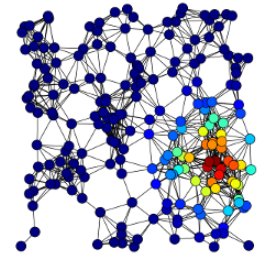
\includegraphics[width=5.5cm]{centrality.png}
    \end{column}
\end{columns}
\end{minipage}
}

%%%%%%%%%%%%%%%%%%%%%%%%%%%%%%%%%%%%%%%%%%%%%%%%%%%%%%%%%%%%%%%%%%%%%%%%%%%%%%%%%%%%%%%%%%%%%%%%%%%%%%%%%%

\frame
{
\frametitle{Example of Physical Features}


\begin{minipage}[0.2\textheight]{\textwidth}
\begin{columns}
    \begin{column}{0.6\textwidth}
    \begin{itemize}
    \item The \textbf{Voronoi cell volume, $v_i$}, is a local density measure. It measures how large the empty space is surrounding an atom $i$.
    \item Standardized cell volume, $\hat{v_i}$, can help filter out the affine displacement introduced by pulling the glass uni-axially.
    \newline
    $$\hat{v_i} = \frac{(v_i - \mu_v)}{\sigma_v}$$
    \newline
    \end{itemize}
    \end{column}
    
    \begin{column}{0.5\textwidth}
%    \vspace{4em}
    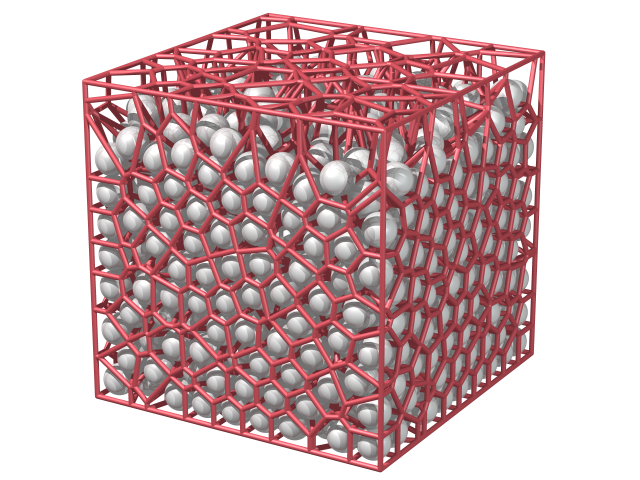
\includegraphics[width=5.5cm]{images/voronoi.png}
    \end{column}
\end{columns}
\end{minipage}
}

%%%%%%%%%%%%%%%%%%%%%%%%%%%%%%%%%%%%%%%%%%%%%%%%%%%%%%%%%%%%%%%%%%%%%%%%%%%%%%%%%%%%%%%%%%%%%%%%%%%%%%%%%%
\frame{

\frametitle{Extracting Ground Truth}

\begin{minipage}[0.2\textheight]{\textwidth}
\begin{columns}[T]
    \begin{column}{0.5\textwidth}
    
    \begin{itemize}
    \begin{footnotesize}
    \item 
    If $\hat{v_i} = \frac{(v_i - \mu_v)}{\sigma_v}$ exceeds a certain threshold, then atom $i$ is defined as part of a nucleation event. We define ground truth label as:
    $$
    y_i = \begin{cases}
      0 & \text{if }{\hat{v_i} \le 3} \\
      1 & \text{if }{\hat{v_i} \ge 3} \\
    \end{cases} 
    $$
    %%%%%%ground truth%%%%%%
    \item A K-nearest-neighbors algorithm will be applied to label those false-negative atoms.
    \end{footnotesize}  
    \end{itemize}
    \end{column}
    
    \begin{column}{0.5\textwidth}
    \vspace{3em}
    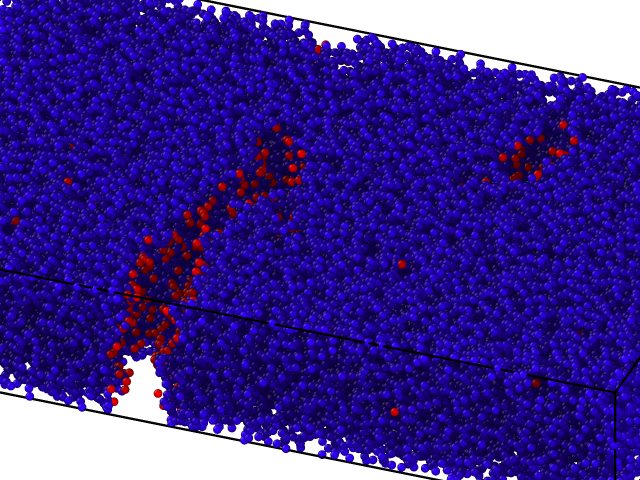
\includegraphics[width=5.5cm]{images/face.png}
    \end{column}
\end{columns}
\end{minipage}
}

%%%%%%%%%%%%%%%%%%%%%%%%%%%%%%%%%%%%%%%%%%%%%%%%%%%%%%%%%%%%%%%%%%%%%%%%%%%%%%%%%%%%%%%%%%%%%%%%%%%%%%%%%%
\subsection{Machine Learning}
\frame{
\frametitle{Machine Learning Methods}

\begin{block}{}
Objective is to produce surrogate model of MD simulations using supervised learning.

\begin{itemize}
    \item Use ensemble-based methods such as {\bf random forest} (RF) to predict nucleation at fixed future time step, given $t=0$ feature values.
    \item Use {\bf recurrent neural networks} (RNN) to learn dynamics of fracture propagation.
\end{itemize}
\end{block}
}

%%%%%%%%%%%%%%%%%%%%%%%%%%%%%%%%%%%%%%%%%%%%%%%%%%%%%%%%%%%%%%%%%%%%%%%%%%%%%%%%%%%%%%%%%%%%%%%%%%%%%%%%%%


\frame{
\frametitle{Ensemble methods}

{\bf Ensemble-based methods} predict atom labels by combining predictions from multiple estimators, learned from training data.

\medskip

\begin{block}{}

\begin{itemize}
    \item Bagging: {\bf random forest}.
    \begin{itemize}
        \item Estimators are decision trees constructed based on feature subsets drawn randomly with replacement.
        \item Labels determined by majority vote among decision trees.
    \end{itemize}
    
    \medskip
    
    \item Boosting: {\bf adaboost}.
    \begin{itemize}
        \item Estimators are classifiers based on individual features.
        \item Labels determined by weighted sum of classifier outputs, 
        weights updated successively to improve prediction accuracy.
    \end{itemize}
\end{itemize}
\end{block}
}
%%%%%%%%%%%%%%%%%%%%%%%%%%%%%%%%%%%%%%%%%%%%%%%%%%%%%%%%%%%%%%%%%%%%%%%%%%%%%%%%%%%%%%%%%%%%%%%%%%%%%%%%%%

\frame{
\frametitle{Recurrent Neural Networks}

RNN trains on an entire time series, learning dynamics of a process which it stores using a ``memory'' of internal states.

\begin{center}
\begin{figure}[!b]

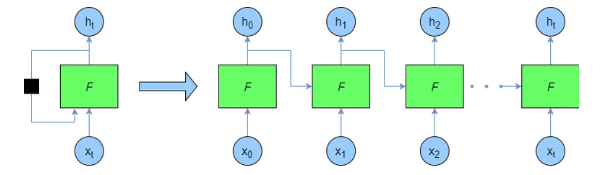
\includegraphics[width=11.5cm , height = 3.5cm]{images/rnn.PNG}

\end{figure}
\end{center}

Training input is time series of features from MD simulation data.
}
%%%%%%%%%%%%%%%%%%%%%%%%%%%%%%%%%%%%%%%%%%%%%%%%%%%%%%%%%%%%%%%%%%%%%%%%%%%%%%%%%%%%%%%%%%%%%%%%%%%%%%%%%%

\frame{
\frametitle{Recurrent Neural Networks}
\begin{block}{}
\begin{itemize}
    \item In training, RNN uses information from all times up to time step $t$, to output feature values and ground truth labels for time $t+1$.
    \begin{itemize}
        \item {\bf Long Short-Term Memory} (LSTM) mechanism gives added weight to information from more recent time steps.
    \end{itemize}
    \item Loss function describes difference between output values and training data.
    \item Neural network weights updated successively, to minimize loss function and improve prediction accuracy.

\end{itemize}
\end{block}
}
%%%%%%%%%%%%%%%%%%%%%%%%%%%%%%%%%%%%%%%%%%%%%%%%%%%%%%%%%%%%%%%%%%%%%%%%%%%%%%%%%%%%%%%%%%%%%%%%%%%%%%%%%%
\frame{
\frametitle{Proposed Architecture}

\begin{center}
\begin{figure}[!b]
    \centering
    \noindent
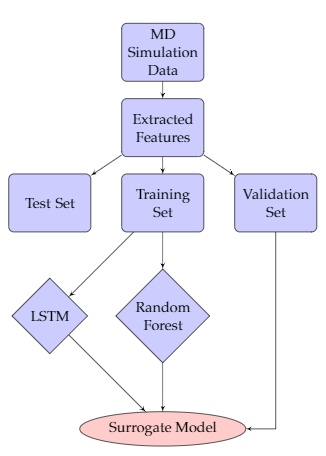
\includegraphics[width=4.5cm , height = 6cm]{images/arch.PNG}

Machine Learning Architecture

\end{figure}
\end{center}

}













%%%%%%%%%%%%%%%%%%%%%%%%%%%%%%%%%%%%%%%%%%%%%%%%%%%%%%%%%%%%%%%%%%%%%%%%%%%%%%%%%%%%%%%%%%%%%%%%%%%%%%%%%%


